\subsubsection*{Le matin :}
Pour résoudre le probleme d'hier, une piste est envisagée :\\
    Avant l'entrainement, les données sont triées.
    Cela premet de créer deux sets different,
    le premier auras une moyene plus faible que le second.
    J'ai aussi ajouté mis le parametre shuffle a False dans l'entrainement du model.


\subsubsection*{L'après midi :}
Le trie avant de passer a l'apprentissage a l'air d'ameliorer les resultats.
Cet après midi a été essentiellement passé a creer des plots pout visualiser les données :
Voici les résultats (moyenne $\pm$ ecart type) de 100 entrainement avec des données trié et non trié.
\begin{figure}[H]
    \center
    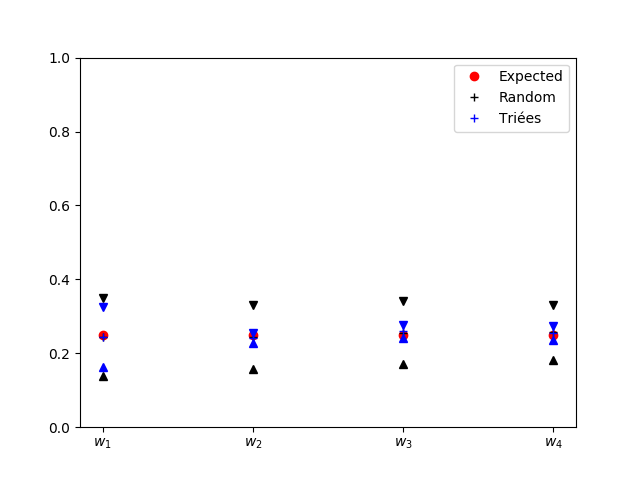
\includegraphics[height=\grand]{sources/data/pbtrie/graph}
	\caption{Apprentissage d'une fonction de choquet}
	\label{pbtrie}
\end{figure}

On peut voir que le trie affecte l'apprentissage, pour mieux savoir a quel point, de nouvelles mesures sont nescessaires.
